\documentclass[11pt,french,french]{article}
\usepackage{lmodern}
\usepackage{amssymb,amsmath}
\usepackage{ifxetex,ifluatex}
\usepackage{fixltx2e} % provides \textsubscript
\ifnum 0\ifxetex 1\fi\ifluatex 1\fi=0 % if pdftex
  \usepackage[T1]{fontenc}
  \usepackage[utf8]{inputenc}
\else % if luatex or xelatex
  \ifxetex
    \usepackage{mathspec}
    \usepackage{xltxtra,xunicode}
  \else
    \usepackage{fontspec}
  \fi
  \defaultfontfeatures{Mapping=tex-text,Scale=MatchLowercase}
  \newcommand{\euro}{€}
\fi
% use upquote if available, for straight quotes in verbatim environments
\IfFileExists{upquote.sty}{\usepackage{upquote}}{}
% use microtype if available
\IfFileExists{microtype.sty}{%
\usepackage{microtype}
\UseMicrotypeSet[protrusion]{basicmath} % disable protrusion for tt fonts
}{}
\usepackage[margin=0.95in]{geometry}
\ifxetex
  \usepackage{polyglossia}
  \setmainlanguage{}
\else
  \usepackage[shorthands=off,french]{babel}
\fi
\usepackage{color}
\usepackage{fancyvrb}
\newcommand{\VerbBar}{|}
\newcommand{\VERB}{\Verb[commandchars=\\\{\}]}
\DefineVerbatimEnvironment{Highlighting}{Verbatim}{commandchars=\\\{\}}
% Add ',fontsize=\small' for more characters per line
\usepackage{framed}
\definecolor{shadecolor}{RGB}{248,248,248}
\newenvironment{Shaded}{\begin{snugshade}}{\end{snugshade}}
\newcommand{\AlertTok}[1]{\textcolor[rgb]{0.94,0.16,0.16}{#1}}
\newcommand{\AnnotationTok}[1]{\textcolor[rgb]{0.56,0.35,0.01}{\textbf{\textit{#1}}}}
\newcommand{\AttributeTok}[1]{\textcolor[rgb]{0.77,0.63,0.00}{#1}}
\newcommand{\BaseNTok}[1]{\textcolor[rgb]{0.00,0.00,0.81}{#1}}
\newcommand{\BuiltInTok}[1]{#1}
\newcommand{\CharTok}[1]{\textcolor[rgb]{0.31,0.60,0.02}{#1}}
\newcommand{\CommentTok}[1]{\textcolor[rgb]{0.56,0.35,0.01}{\textit{#1}}}
\newcommand{\CommentVarTok}[1]{\textcolor[rgb]{0.56,0.35,0.01}{\textbf{\textit{#1}}}}
\newcommand{\ConstantTok}[1]{\textcolor[rgb]{0.00,0.00,0.00}{#1}}
\newcommand{\ControlFlowTok}[1]{\textcolor[rgb]{0.13,0.29,0.53}{\textbf{#1}}}
\newcommand{\DataTypeTok}[1]{\textcolor[rgb]{0.13,0.29,0.53}{#1}}
\newcommand{\DecValTok}[1]{\textcolor[rgb]{0.00,0.00,0.81}{#1}}
\newcommand{\DocumentationTok}[1]{\textcolor[rgb]{0.56,0.35,0.01}{\textbf{\textit{#1}}}}
\newcommand{\ErrorTok}[1]{\textcolor[rgb]{0.64,0.00,0.00}{\textbf{#1}}}
\newcommand{\ExtensionTok}[1]{#1}
\newcommand{\FloatTok}[1]{\textcolor[rgb]{0.00,0.00,0.81}{#1}}
\newcommand{\FunctionTok}[1]{\textcolor[rgb]{0.00,0.00,0.00}{#1}}
\newcommand{\ImportTok}[1]{#1}
\newcommand{\InformationTok}[1]{\textcolor[rgb]{0.56,0.35,0.01}{\textbf{\textit{#1}}}}
\newcommand{\KeywordTok}[1]{\textcolor[rgb]{0.13,0.29,0.53}{\textbf{#1}}}
\newcommand{\NormalTok}[1]{#1}
\newcommand{\OperatorTok}[1]{\textcolor[rgb]{0.81,0.36,0.00}{\textbf{#1}}}
\newcommand{\OtherTok}[1]{\textcolor[rgb]{0.56,0.35,0.01}{#1}}
\newcommand{\PreprocessorTok}[1]{\textcolor[rgb]{0.56,0.35,0.01}{\textit{#1}}}
\newcommand{\RegionMarkerTok}[1]{#1}
\newcommand{\SpecialCharTok}[1]{\textcolor[rgb]{0.00,0.00,0.00}{#1}}
\newcommand{\SpecialStringTok}[1]{\textcolor[rgb]{0.31,0.60,0.02}{#1}}
\newcommand{\StringTok}[1]{\textcolor[rgb]{0.31,0.60,0.02}{#1}}
\newcommand{\VariableTok}[1]{\textcolor[rgb]{0.00,0.00,0.00}{#1}}
\newcommand{\VerbatimStringTok}[1]{\textcolor[rgb]{0.31,0.60,0.02}{#1}}
\newcommand{\WarningTok}[1]{\textcolor[rgb]{0.56,0.35,0.01}{\textbf{\textit{#1}}}}
\ifxetex
  \usepackage[setpagesize=false, % page size defined by xetex
              unicode=false, % unicode breaks when used with xetex
              xetex]{hyperref}
\else
  \usepackage[unicode=true]{hyperref}
\fi
\hypersetup{breaklinks=true,
            bookmarks=true,
            pdfauthor={},
            pdftitle={},
            colorlinks=true,
            citecolor=blue,
            urlcolor=blue,
            linkcolor=magenta,
            pdfborder={0 0 0}}
\urlstyle{same}  % don't use monospace font for urls
\setlength{\parindent}{0pt}
\setlength{\parskip}{6pt plus 2pt minus 1pt}
\setlength{\emergencystretch}{3em}  % prevent overfull lines
\setcounter{secnumdepth}{5}

%%% Use protect on footnotes to avoid problems with footnotes in titles
\let\rmarkdownfootnote\footnote%
\def\footnote{\protect\rmarkdownfootnote}


  \title{Analyse statistique et empirique des modèles\\
de Word Embedding sur Twitter}
    \author{Kim Antunez, Romain Lesauvage, Alain Quartier-la-Tente\\
sous l'encadrement de Benjamin Muller (Inria)}
    \date{}
  
\usepackage{caption}
\usepackage{graphicx}
\usepackage{natbib}
\usepackage[dvipsnames]{xcolor}

\begin{document}

\maketitle


\hypertarget{partie-1}{%
\section{Partie 1}\label{partie-1}}

\label{sec:word2vec}

\hypertarget{uxe9valuation-du-moduxe8le-impluxe9mentuxe9}{%
\section{Évaluation du modèle
implémenté}\label{uxe9valuation-du-moduxe8le-impluxe9mentuxe9}}

\hypertarget{comment-uxe9valuer-le-moduxe8le}{%
\subsection{Comment évaluer le modèle
?}\label{comment-uxe9valuer-le-moduxe8le}}

\label{sec:comment_evaluer}

Malgré l'utilisation généralisée des \emph{word embedding}, très peu de
travaux théoriques expliquent ce qui est réellement capturé par ces
représentations de mots.

C'est pourquoi ce modèle est principalement évalué à l'aide de méthodes
empiriques. Nous allons décrire dans cette partie
\ref{sec:comment_evaluer} quelques méthodes que nous avons retenues pour
évaluer la qualité des vecteurs-mots obtenus.

\hypertarget{distance-entre-deux-mots}{%
\subsubsection{Distance entre deux
mots}\label{distance-entre-deux-mots}}

L'un des enjeux principaux du modèle étant de pouvoir estimer la
proximité entre deux vecteurs-mots, nous pouvons tout d'abord mesurer
cette dernière par des calculs de distance.

Il existe différents types de distances. Chacune d'elles possède des
propriétés intéressantes et s'adaptent plus ou moins bien au problème
traité. Nous avons ici retenu deux distances classiquement utilisées :

\begin{itemize}
\item \textbf{la distance euclidienne} $ d_{e}(\vec{u},\vec{v}) = \left\| \vec{u} - \vec{v}  \right\|_2$

La longueur du vecteur mot, captée dans le cas de la distance euclidienne, est positivement corrélée à la fréquence d'apparition du mot (\cite{Schakel}). Cette information peut s'avérer utile dans l'analyse de la signification des mots, notamment lorsque l'on effectue des opérations sur les vecteurs (comme l'exemple de $\overrightarrow{Paris} - \overrightarrow{France} + \overrightarrow{Italie} = \overrightarrow{Rome}$ dans \cite{Mikolov})

Toutefois, cette dépendance à la fréquence d'apparition peut également fausser l'analyse. C'est pourquoi nous avons choisi, par la suite, de normaliser les vecteurs. 

$ d_{e}(\vec{u},\vec{v}) = \left\| \frac{\vec{u}}{\left\| \vec{u} \right\|_2} - \frac{\vec{v}}{\left\| \vec{v} \right\|_2}  \right\|_2$


\item \textbf{la similarité cosinus} $ d_{c}(\vec{u}, \vec{v}) = \frac{\vec{u}.\vec{v}}{\left\| \vec{u} \right\|_2  \left\| \vec{v} \right\|_2 }$.

La similarité cosinus correspond au produit scalaire entre les deux vecteurs normalisés. Elle mesure ainsi l'angle formé entre deux vecteurs-mots.

C'est la distance que de nombreux papiers fondateurs de la méthode \emph{Word2Vec} (comme \cite{Mikolov} ou \cite{Levy}) utilisent avec l'argument selon lequel les mots apparaissant dans des contextes similaires sont groupés dans la même direction durant l'entraînement. 
Une similarité est proche de +1 si deux mots sont positivement reliés (proches), de -1 s'ils sont négativement reliés (éloignés) et de 0 s'ils ne sont pas \og reliés \fg. 

Il est toutefois délicat d'interpréter une similarité proche de -1. On pourrait intuitivement penser à des antonymes, comme \og grand \fg et \og petit \fg, mais en pratique, les antonymes sont susceptibles d'apparaître dans des contextes semblables et sont donc bien souvent positivement corrélés. 

 
\end{itemize}

\hypertarget{analyse-en-composantes-principales}{%
\subsubsection{Analyse en Composantes
Principales}\label{analyse-en-composantes-principales}}

Une fois le modèle \emph{Word2Vec} entraîné, nous obtenons des
\emph{word-embeddings} pour chacun de nos mots, représentés par des
vecteurs de grandes dimensions (20, 50 ou même supérieures à 100).

Dès lors, il devient complexe de bien observer la proximité entre deux
mots. C'est pourquoi il devient utile de mobiliser des méthodes de
réduction de dimensions comme l'analyse en composantes principales
(ACP). L'objectif premier de cette méthode est en effet de projeter un
nuage de points sur un espace de dimension inférieure afin de rendre
l'information moins redondante et plus visuelle, tout en étant le plus
proche possible de la réalité.

Considérons le cas où nous disposons de \(n\) individus (dans notre cas
les mots) et de \(p\) variables (dans notre cas, leurs composantes ou
dimensions issues du modèle \emph{Word2Vec}). On note \(X = (x_{ij})\)
la matrice de taille \((n,p)\) des données brutes, où \(x_{ij}\)
représente la valeur de la \(j\)-ème variable pour le \(i\)-ème
individu. Afin de donner à chaque individu le même poids, nous centrons
et réduisons les colonnes de notre matrice de données. On notera par la
suite \(Z = (z_{ij})\) la matrice des données centrées et réduites.

La construction des axes de l'ACP est faite par projection orthogonale.
Nous utilisons ici le produit scalaire \(<x,y>_{N} = x\,^t N y\) avec la
métrique \(N = diag(\frac{1}{n},...,\frac{1}{n})\). Ainsi, la projection
orthogonale d'un individu i (vecteur ligne) \(z_i\) sur une droite de
vecteur directeur \(v\) vaut \(^tz_iv\) et les coordonnées de projection
des \(n\) individus valent \(Zv\).

Les vecteurs directeurs des axes sont définis de manière à maximiser la
dispersion du nuage (son inertie) des individus projetés et conserver
ainsi au mieux les distances entre les individus. L'inertie se définit
comme

\[I(Z) = \frac{1}{n} \sum \limits_{i = 1}^n d_{e}^2(z_i,\bar{z}) = \sum \limits_{i = 1}^n var(z^j) = p\]

avec \(d_{e}(z_i,z_{i'})\) la distance euclidienne entre deux individus
\(z_i\) et \(z_{i'}\) :
\(d_{e}(z_i,z_{i'}) = \sum \limits_{j=1}^p (z_{ij} - z_{i'j})^2\)\footnote{Nous
  travaillons ici dans le cadre d'une ACP normée où la matrice \(X\) a
  été centrée puis réduite. La réduction de \(X\) a modifié les
  distances initiales entre individus
  (\(d_{e}(z_i,z_{i'}) \neq d_{e}(x_i,x_{i'})\)). Cela n'aurait pas été
  le cas si la matrice \(Y\) avait été uniquement centrée (ACP non
  normée).}.

On trouve tout d'abord le vecteur directeur \(v_1\) qui orientera le
premier axe de l'ACP grâce au programme suivant :
\[v_1 =\underset{\Vert v \Vert = 1}{\mathrm{argmax~}} Var(Zv) =\underset{\Vert v \Vert = 1}{\mathrm{argmax~}} v\,^t R v \]
où \(R = Var(Z) = \frac{1}{n} Z\,^t Z\) est la matrice des corrélations
entre les p variables. La norme du vecteur \(v\) se calcule dans ce
nouvel espace comme
\(\Vert v \Vert = \sqrt{<v,v>} = v ^tv =\sqrt{ \sum \limits_{i = 1}^p v_i^2}\)

Puis, on choisit \(v_2\) orthogonal à \(v_1\) tel que l'inertie soit
toujours maximisée
\[v_2 =\underset{ \Vert v \Vert = 1,\,v \perp v_1}{\mathrm{argmax}}\;  Var(Zv) \]
En procédant de manière séquentielle, on obtient \(q < r\) axes
orthogonaux avec \(r = rg(Z)\) et \(q\) choisi par le
statisticien\footnote{Différentes méthodes existent afin de déterminer
  le \(q\) optimal, comme la règle de Kaiser ou encore celle du coude.}.

On peut montrer que \(\forall k < q\) :

\begin{itemize}
\item $v_k$ est un vecteur propre associé à la k\ieme{} valeur propre $\lambda_k$ de $R$
\item la composante principale $Zv_k$ est centrée et $V(Zv_k)= \lambda_k$
\item Les $Zv_k$ ne sont pas corrélés entre eux
\end{itemize}

On obtient alors la matrice \(F = ZV\) des nouvelles coordonnées
factorielles des individus, avec \(V = (v_1,\dots,v_q)\) la matrice des
vecteurs propres.

Nous utilisons ici l'ACP en vue d'identifier les individus (ici, nos
mots) qui sont proches. Pour ce faire, il suffit de représenter les
coordonnées factorielles de la matrice \(F\) dans des repères, en
général en 2 dimensions pour une question de lisibilité. Deux mots
apparaissant dans des contextes similaires seront proches sur ce repère
et orientés dans la même direction.

Enfin, pour juger de la qualité de la réduction de dimension, on calcule
souvent la proportion de l'inertie totale expliquée par les \(q\)
premières composantes principales.

\[ \frac{V(F)}{I(Z)} = \frac{\sum \limits_{i = 1}^q \lambda_i}{p}\]

\hypertarget{algorithme-t-distributed-stochastic-neighbor-embedding}{%
\subsubsection{Algorithme t-distributed Stochastic Neighbor
Embedding}\label{algorithme-t-distributed-stochastic-neighbor-embedding}}

Bien que l'ACP soit une première manière de résumer l'information
contenue dans nos vecteurs, elle présente des limites, notamment dans
les vecteurs aux trop grandes dimensions, pour lesquels l'inertie des
premiers axes de l'ACP peut se révéler faible.

Pour combler ces lacunes, un autre algorithme de réduction de dimension
peut être utilisé, celui dit du t-distributed Stochastic Neighbor
Embedding. Contraitement à l'ACP, cet algorithme est stochastique et
non-linéaire et il favorise l'apparition de groupes de mots proches. Sa
philosophie demeure cependant identique : représenter dans un espace à
dimension réduite notre nuage de points de manière à repérer les mots
proches.

La première étape de l'algorithme consiste à calculer les similarités
entre les \(n\) vecteurs-mots \((x_i)_{i=1...n}\). La similarité entre
\(x_i\) et \(x_j\) se mesure comme étant la probabilité conditionnelle
\(p_{j|i}\) de choisir \(x_j\) comme voisin de \(x_i\), si les voisins
étaient tirés au sort selon une loi
\(\mathcal{N}(x_i, \sigma_i)\)\footnote{\(\sigma_i\) doit être calculé
  de manière à adapter la loi conditionnelle aux données. Une faible
  dispersion autour de \(x_i\) entraînera un \(\sigma_i\) faible et
  réciproquement. Il s'agit de trouver le \(\sigma_i\) qui minimise ce
  qui est appelé en théorie de l'information la \og perplexité \fg,
  c'est-à-dire un indicateur qui décrit à quel point une distribution de
  probabilité réussit à prédire un échantillon.}

\[ p_{j|i} = \frac{\exp({-\frac{(d_e(x_i - x_j))^2}{2\sigma_i^2})}}{\sum_{k \neq i}{\exp({-\frac{(d_e(x_i - x_k))^2}{2\sigma_i^2})}}}\]

La seconde étape de l'algorithme consiste à trouver le nouvel espace de
projection à faible nombre de dimensions. On appellera \(g_i\) les
\(x_i\) projetés dans cet espace que l'on cherche à déterminer. De la
même manière que précédemment, on exprime des probabilité
conditionnelles \(q_{j|i}\) en fonction des \(g_i\) mais qui suivent
cette fois-ci une distribution de \emph{Student} - d'où le nom de
l'algorithme - plutôt qu'une loi gaussienne\footnote{Dans un espace à
  faible dimension, la dispersion des vecteurs est réduite. La
  distribution de Student possède des queues plus épaisses que la loi
  normale, ce qui permet de mieux différencier les vecteurs distants des
  vecteurs similaires.}.

\[ q_{j|i} = \frac{(1+ (d_e(g_i - g_j))^2)^{-1}}{\sum_{k \neq i}{(1+ (d_e(g_i - g_k))^2)^{-1}}}\]

Afin d'obtenir les \(g_i\), on minimise, par descente de gradient, la
divergence de Kullback--Leibler entre les distributions de probabilité P
et Q :

\[KL(P,Q) = \sum_{i \neq j} { p_{ij} \log{\frac{p_{ij}}{q_{ij}}}} \qquad\text{avec}\qquad p_{ij} = \frac{p_{i|j} + p_{j|i}}{2n}\]

Comme dans l'algorithme de l'ACP, l'algorithme de t-SNE nous permet
d'obtenir une nouvelle projection des \(x_i\). Il faut cependant
analyser avec précaution ses résultats. L'algorithme n'étant pas
linéaire, l'interprétation de la taille des \emph{clusters} obtenus ou
de la distance qui les sépare n'est alors pas directe.

\hypertarget{jugement-humain}{%
\subsubsection{Jugement humain}\label{jugement-humain}}

\label{sec:jugement_humain}

Les \emph{word-embedding} obtenus par \emph{Word2Vec} sont censés
regrouper les mots qui apparaissent dans un contexte similaire. Une
dernière façon de le vérifier peut être de comparer les résultats
obtenus au point de vue des êtres humains sur la proximité qu'il peut y
avoir entre différentes paires de mots.

Pour ce faire, nous utilisons une base de données d'une soixantaine de
paires de mots auxquelles sont associés des scores de similarité allant
de 0 (aucun lien entre les mots) à 4 (mots identiques).

\begin{tabular}{|c|c|c|}
    \hline
    mot 1 & mot 2 & similarité  \tabularnewline
    \hline
    corde & sourire & 0,00   \tabularnewline
    midi & ficelle & 0,00   \tabularnewline
    \dots & \dots & \dots   \tabularnewline
    corde & ficelle & 3,33   \tabularnewline
    \dots & \dots & \dots   \tabularnewline
    automobile & auto & 3,94   \tabularnewline
    coq & coq & 4,00   \tabularnewline
    \hline
 \end{tabular}

Nous calculons ensuite la corrélation de Spearman entre les similarités
cosinus de ces différentes paires issues de notre modèle (notées ici
\((X_i)_{i=1..n}\)) et les scores proposés ci-dessus par des êtres
humains (notés ici \((Y_i)_{i=1..n}\)).

La corrélation de Spearman est égale au coefficient de corrélation de
Pearson calculé sur les variables de rang. \[
r_s = \mathrm{corr}(\mathrm{rg}_X, \mathrm{rg}_Y) = 
\frac{\mathrm{cov}(\mathrm{rg}_X, \mathrm{rg}_Y)}{
\sigma_{\mathrm{rg}_X} \sigma_{\mathrm{rg}_Y}
}
\] La variable de rang \(\mathrm{rg}_{X_i}\) est définie telle que
\(\mathrm{rg}_{X_i}=j \iff X_i = X_{(j)}\) (\(X_i\) est la \(j\)ème plus
petite variable).

Pour tester la significativité de ce coefficient, nous réalisons un test
de Student avec

\[t = r\sqrt{\frac{n-2}{1-r^2}}\overset{H_0}{\sim} St(n-2)\]

\colorbox{BurntOrange}{Speech sur intervalle de confiance}

\hypertarget{evaluation-sur-un-corpus-fictif}{%
\subsection{Evaluation sur un corpus
fictif}\label{evaluation-sur-un-corpus-fictif}}

\label{sec:corpus_fictif}

Avant de nous attaquer au jeu de données complet, nous avons évalué un
premier corpus fictif afin de nous assurer de la robustesse du modèle
implémenté. Nous avons associé dix couples (du type {[}voiture,
camion{]}), à dix mots contexte différents ({[}véhicule, moto,
\dots{]}). Le corpus fictif est formé de 10 000 phrases composées
chacune d'un mot d'un couple, de cinq mots du contexte et de trois mots
bruits, tous tirés aléatoirement.

Nous avons ensuite mis en œuvre les différentes techniques
d'évaluation{[}à l'exception de la méthode par \og jugement humain
\fg puisque le corpus est ici créé fictivement par ordinateur sans
prêter attention au réel sens des mots.{]} présentées en partie
\ref{sec:comment_evaluer} sur ce corpus fictif.

\begin{figure}[!ht]
\begin{center}
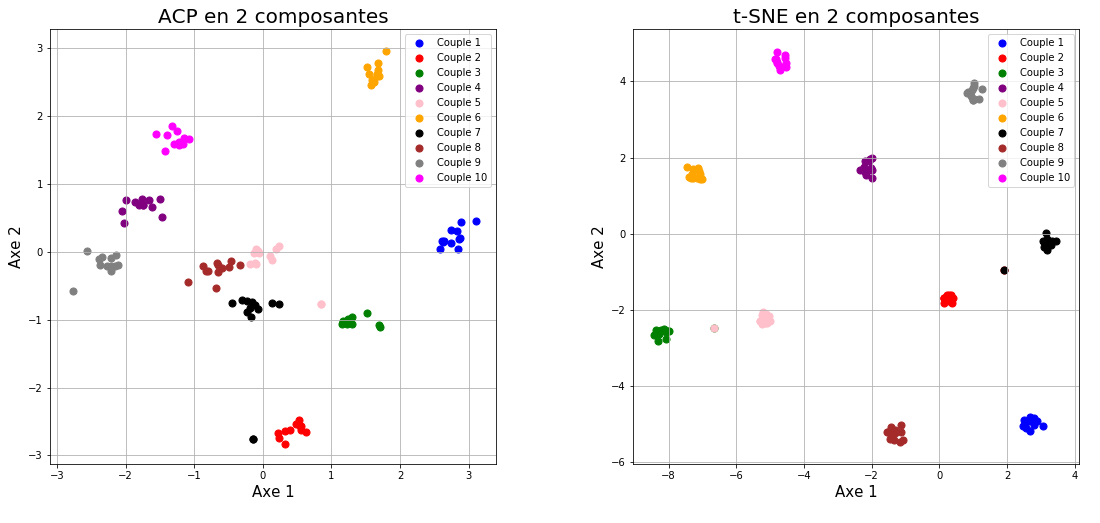
\includegraphics[width=1\textwidth]{img/figures.png}
\captionsetup{margin=0cm,format=hang,justification=justified}
\caption{Évaluation du modèle sur données fictives}\label{fig:figure_evaluation}
\end{center}
\vspace{-0.3cm}
\footnotesize
\emph{Note : Paramètres utilisés : epochs = 50 / lr = 0,01 / window = 5 / dim = 10.}
\end{figure}

Les résultats semblent concluants : la similarité cosinus montre bien
une forte corrélation entre les mots focus et contexte du corpus initial
et une faible corrélation avec les mots bruits. L'ACP et l'algorithme
t-SNE permettent également de montrer graphiquement cette proximité
(figure \ref{fig:figure_evaluation}). L'algorithme t-SNE semble bien
discriminer davantage les clusters que l'ACP.

\begin{Shaded}
\begin{Highlighting}[]
\KeywordTok{mot_plus_proche}\NormalTok{(}\StringTok{"grand"}\NormalTok{, }\DataTypeTok{n =} \DecValTok{50}\NormalTok{)}
\CommentTok{#[('énorme', 0.9914256427481623),}
\CommentTok{# ('taille', 0.9905528713008166),}
\CommentTok{# […]}
\CommentTok{# ('vanille', 0.06068283530950071),}
\CommentTok{# ('salissures', 0.0539210063101789)]}
\end{Highlighting}
\end{Shaded}

\hypertarget{choix-des-meilleurs-hyperparamuxe8tres-pour-le-moduxe8le}{%
\subsection{Choix des meilleurs hyperparamètres pour le
modèle}\label{choix-des-meilleurs-hyperparamuxe8tres-pour-le-moduxe8le}}

Une fois nous être assurés de la bonne implémentation du modèle (partie
\ref{sec:corpus_fictif}) grâce au corpus fictif, nous nous sommes
attachés à identifier les hyperparamètres les plus pertinents au regard
des données dont nous disposons.

Le modèle word2vec version CBOW, décrit en partie \ref{sec:word2vec},
fait en effet intervenir un certain nombre d'hyperparamètres\footnote{les
  paramètres en gras sont ceux dont nous avons évalué l'effet} :

\begin{itemize}
\item \textbf{$\alpha$ : le \og \emph{learning rate} \fg, ou taux d'apprentissage}
\item \textbf{$window$ : la taille de la fenêtre de sélection des mots contextes}
\end{itemize}

\colorbox{BurntOrange}{Compléter après lecture partie Alain et harmoniser le nom des hyperparamètres dans l'ensemble du rapport.}

Or, la performance de nombreuses méthodes de \emph{machine learning},
dont Word2Vec, dépend fortement des valeurs choisies pour les
hyperparamètres, ces dernières dépendant directement des données
mobilisées.

Même si les méthodes d'optimisation bayésiennes deviennent de plus en
plus performantes pour optimiser la valeur de ces hyperparamètres et de
leurs interactions (\cite{Hutter}), le choix de ces paramètres
s'effectue régulièrement de manière empirique, en testant différentes
valeurs sur les données mobilisées. C'est l'approche que nous retenons
ici.

\hypertarget{utilisation-du-moduxe8le-gensim}{%
\subsubsection{\texorpdfstring{Utilisation du modèle
\texttt{Gensim}}{Utilisation du modèle Gensim}}\label{utilisation-du-moduxe8le-gensim}}

Le package \texttt{Gensim} (\og Generate Similar \fg), dans lequel la
méthode \emph{Word2Vec} est implémentée, est un des outils actuels les
plus robustes et performants\footnote{Grâce à sa dépendance à
  \texttt{NumPy}, \texttt{Gensim} puise dans des bibliothèques de bas
  niveau. Ainsi, alors que le code de haut niveau est du Python, c'est
  en fait du Fortran et du C hautement optimisés qui sont utilisés, ce
  qui rend \texttt{Gensim} bien plus performant que \texttt{PyTorch} que
  nous utilisons.} pour de modélisation sémantique non supervisée
(\cite{Rehurek}).

Nous avons choisi de mobiliser \texttt{Gensim} dans la suite de ce
rapport, en parallèle du modèle que nous avons implémenté, en raison de
son exécution bien plus rapide\footnote{A titre d'exemple, alors qu'une
  epoch sur l'ensemble des tweets met une vingtaine d'heures à tourner
  pour \og notre \fg modèle, elle met \colorbox{BurntOrange}{X minutes}
  via \texttt{Gensim}.}. Cette rapidité d'exécution nous a permis de
réaliser de plus nombreux tests d'hyperparamètres que nous vous
présentons ici.

Afin de tester l'effet des différentes valeurs des hyperparamètres, nous
avons fait tourner le modèle \emph{Word2Vec} plusieurs fois en modifiant
un à un les paramètres. Nous avons ensuite évalué ces différents modèles
par la méthode du \og jugement humain \fg (cf.~partie
\ref{sec:jugement_humain}). En outre, un même modèle est lancé six fois
(six \og seeds \fg différentes) afin de construire des intervalles de
confiance de la matière décrite précédemment.

\hypertarget{sur-de-notre-moduxe8le}{%
\subsubsection{\texorpdfstring{Sur de \og notre
\fg modèle}{Sur de notre modèle}}\label{sur-de-notre-moduxe8le}}

\colorbox{BurntOrange}{TODO : comparer en espérant que ça 
 donne des résultats à peu près semblables à Gensim.}

\hypertarget{evaluation-sur-le-corpus-final}{%
\subsection{Evaluation sur le corpus
final}\label{evaluation-sur-le-corpus-final}}

\colorbox{BurntOrange}{Montrer les 4 évaluation du corpus final de 1 000 000 de tweets.
 Dire en quoi le modèle semble bon, en quoi il semble pas bon
 (du style bon pour prédire les jours de la semaine, etc. ). }

\nocite{*}

\begin{thebibliography}{999}
\bibitem[Bortoli, C., \emph{et al} (2015)]{Schakel} Schakel, A. M., Wilson, B. J. (2015). Measuring Word Significanceusing Distributed Representations of Words. arXiv:1508.02297. \url{https://arxiv.org/pdf/1508.02297v1.pdf}.
\bibitem[Hutter, F., \emph{et al} (2014)]{Hutter} Hutter, F., Hoos, H., Leyton-Brown, K., (2014). An Efficient Approach for Assessing Hyperparameter Importance. PMLR 32(1):754-762. \url{http://proceedings.mlr.press/v32/hutter14.pdf}.
\bibitem[Levy, O., Golberg, Y. (2015)]{Levy} Levy, O., Golberg, Y. (2015). Neural Word Embedding as Implicit Matrix Factorization.
\url{https://papers.nips.cc/paper/5477-neural-word-embedding-as-implicit-matrix-factorization.pdf}.
\bibitem[Mikolov, T., \emph{et al} (2013)]{Mikolov} Mikolov, T.,  Chen, K., Corrado, G., Dean, J. (2013). Efficient Estimation of Word Representations in Vector Space. arXiv:1301.3781. \url{https://arxiv.org/pdf/1301.3781.pdf}.
\bibitem[{\v R}eh{\r u}{\v r}ek, R., \emph{et al} (2010)]{Rehurek} {\v R}eh{\r u}{\v r}ek, R.,  Sojka, P. (2010). Software Framework for Topic Modelling with Large Corpora. Proceedings of LREC 2010 workshop New Challenges for NLP Frameworks. p. 46--50, 5 pp. ISBN 2-9517408-6-7. \url{https://is.muni.cz/publication/884893/en}.
\end{thebibliography}

\end{document}